\documentclass[
  bibliography=totoc,     % Literatur im Inhaltsverzeichnis
  captions=tableheading,  % Tabellenüberschriften
  titlepage=firstiscover, % Titelseite ist Deckblatt
]{scrartcl}

% Paket float verbessern
\usepackage{scrhack}

\setlength{\parindent}{0em}

% Warnung, falls nochmal kompiliert werden muss
\usepackage[aux]{rerunfilecheck}

% unverzichtbare Mathe-Befehle
\usepackage{amsmath}
% viele Mathe-Symbole
\usepackage{amssymb}
% Erweiterungen für amsmath
\usepackage{mathtools}

% Fonteinstellungen
\usepackage{fontspec}
% Latin Modern Fonts werden automatisch geladen
% Alternativ zum Beispiel:
%\setromanfont{Libertinus Serif}
%\setsansfont{Libertinus Sans}
%\setmonofont{Libertinus Mono}

% Wenn man andere Schriftarten gesetzt hat,
% sollte man das Seiten-Layout neu berechnen lassen
\recalctypearea{}

% deutsche Spracheinstellungen
\usepackage{polyglossia}
\setmainlanguage{german}


\usepackage[
  math-style=ISO,    % ┐
  bold-style=ISO,    % │
  sans-style=italic, % │ ISO-Standard folgen
  nabla=upright,     % │
  partial=upright,   % ┘
  warnings-off={           % ┐
    mathtools-colon,       % │ unnötige Warnungen ausschalten
    mathtools-overbracket, % │
  },                       % ┘
]{unicode-math}

% traditionelle Fonts für Mathematik
\setmathfont{Latin Modern Math}
% Alternativ zum Beispiel:
%\setmathfont{Libertinus Math}

\setmathfont{XITS Math}[range={scr, bfscr}]
\setmathfont{XITS Math}[range={cal, bfcal}, StylisticSet=1]

% Zahlen und Einheiten
\usepackage[
  locale=DE,                   % deutsche Einstellungen
  separate-uncertainty=true,   % immer Fehler mit \pm
  per-mode=symbol-or-fraction, % / in inline math, fraction in display math
]{siunitx}

% chemische Formeln
\usepackage[
  version=4,
  math-greek=default, % ┐ mit unicode-math zusammenarbeiten
  text-greek=default, % ┘
]{mhchem}

% richtige Anführungszeichen
\usepackage[autostyle]{csquotes}

% schöne Brüche im Text
\usepackage{xfrac}

% Standardplatzierung für Floats einstellen
\usepackage{float}
\floatplacement{figure}{htbp}
\floatplacement{table}{htbp}

% Floats innerhalb einer Section halten
\usepackage[
  section, % Floats innerhalb der Section halten
  below,   % unterhalb der Section aber auf der selben Seite ist ok
]{placeins}

% Seite drehen für breite Tabellen: landscape Umgebung
\usepackage{pdflscape}

% Captions schöner machen.
\usepackage[
  labelfont=bf,        % Tabelle x: Abbildung y: ist jetzt fett
  font=small,          % Schrift etwas kleiner als Dokument
  width=0.9\textwidth, % maximale Breite einer Caption schmaler
]{caption}
% subfigure, subtable, subref
\usepackage{subcaption}

% Grafiken können eingebunden werden
\usepackage{graphicx}
% größere Variation von Dateinamen möglich
\usepackage{grffile}

% schöne Tabellen
\usepackage{booktabs}

% Verbesserungen am Schriftbild
\usepackage{microtype}

% Literaturverzeichnis
\usepackage[
  backend=biber,
]{biblatex}
% Quellendatenbank
\addbibresource{lit.bib}
\addbibresource{programme.bib}

% Hyperlinks im Dokument
\usepackage[
  unicode,        % Unicode in PDF-Attributen erlauben
  pdfusetitle,    % Titel, Autoren und Datum als PDF-Attribute
  pdfcreator={},  % ┐ PDF-Attribute säubern
  pdfproducer={}, % ┘
]{hyperref}
% erweiterte Bookmarks im PDF
\usepackage{bookmark}

% Trennung von Wörtern mit Strichen
\usepackage[shortcuts]{extdash}

\author{%
  Sara Krieg\\%
  \href{mailto:sara.krieg@udo.edu}{sara.krieg@udo.edu}%
  \texorpdfstring{\and}{,}%
  Marek Karzel\\%
  \href{mailto:marek.karzel@udo.edu}{marek.karzel@udo.edu}%
}
\publishers{TU Dortmund – Fakultät Physik}


\begin{document}
\maketitle    
\tableofcontents
\newpage
\section{Zielsetzung}
Ziel dieses Versuches ist es, die Absorption von $\gamma$- und $\beta$- Strahlung in verschiedenen Materialien zu untersuchen.
Außerdem wird die Maximalenergie einer $\beta$-Strahlungsquelle bestimmt.

\section{Theorie}
Tritt Strahlung in Materie ein, so nimmt ihre Intensität durch Wechselwirkungen mit den Teilchen im Material ab. Ein Maß für die Häufigkeit
der Wechselwirkungen ist der Wirkungsquerschnitt $\sigma$. Für ein Material der Dicke $D$ mit einem Querschnitt $F$ und einer Teilchendichte
$n$ pro Volumeneinheit ist die Wahrscheinlichkeit für eine Wechselwirkung zwischen einem eintretendem Teilchen mit dem Materials gegeben
durch 
\begin{equation}
W=nD\sigma \quad .
\end{equation}
Treffen $N$ Teilchen pro Zeiteinheit auf die Fläche $F$ so finden demnach
\begin{equation}
N=N_0nD\sigma
\end{equation}
Wechselwirkungen pro Zeiteinheit statt.
Das exponentielle Absoprtionsgesetz
\begin{equation}
N(D)=N_0 \symup{e}^{-\mu D}
\end{equation}
gibt die Anzahl an Teilchen an, die nach Durchgang durch einen Absorber übrigbleiben. Dieses Gesetz gilt unter der Voraussetzung, dass
jedes Teilchen nur einmal wechselwirken kann und dabei vernichtet wird. Der \textit{Absorptionskoeffizient} $\mu$ ist hierbei ein Maß für die Absorptionsstärke
des Materials und ist gegeben durch
\begin{equation}
    \mu =n \cdot \sigma\;.
\end{equation}
Die Schichtdicke, bei welcher die Intensität halbiert wurde, ist gegeben durch
\begin{equation}
D_{\frac{1}{2}}=\frac{\ln(2)}{\mu}\quad .
\end{equation}
Die Anzahl der Teilchen, welche sich im Absorber befinden beträgt
\begin{equation}
n=\frac{z N_{\symup{A}}}{V_{\symup{Mol}}}=\frac{Z N_{\symup{A}}\rho}{M}\quad .
\end{equation}
Hierbei ist $Z$ die Ordnungszahl, $N_{\text{A}}$ die Avogadrokonstante, $V_{\symup{Mol}}$ das Molvolumen und $M$ die molare Masse.
Somit ergibt sich für den Wirkungsquerschnitt $\sigma$
\begin{equation}
\sigma=\frac{\mu}{n}=\frac{\mu M}{Z N_{\symup{A}}\rho} \quad .
\end{equation}

\subsection{\texorpdfstring{$\gamma$}{}-Strahlung}
Fällt ein angeregter Atomkern in einen energetisch niedrigeren Zustand, so werden $\gamma$-Quanten bzw. Photonen emittiert. Die Energie eines
Photons ist dann genau die Differenz der beiden Energieniveaus des Atomkerns
\begin{equation}
E_{\gamma}=E_1-E_2 \quad.
\end{equation}
Da die Energie eines Atomkerns nur diskrete Werte annehmen kann, ergibt sich ein diskreten Linienspektrum des $\gamma$-Strahlers.
Photonen können, da sie sich mit Lichtgeschwindigkeit ausbreiten und demnach keine Ruhemasse besitzen können, keine Teilchen im klassischen Sinne sein.
Tatsächlich weisen sie einige für elektromagnetische Wellen typische Eigenschaften, wie beispielsweise Interferenz, auf. Gemäß der Quantentheorie sind dann Wellenlänge
$\lambda$ und Frequenz $\nu$ der $\gamma$-Strahlung gegeben durch
\begin{equation}
E_{\gamma}=h\nu=\frac{hc}{\lambda}\quad .
\end{equation}

In Materie können Photonen auf unterschiedliche Arten mit dem Material wechselwirken. Die dabei auftretenden Effekte sind in Tabelle \ref{tab:ttab1} aufgeführt.
\FloatBarrier
\begin{table}[h]
    \centering
    \caption{Verschiedene Wechselwirkungen von Photonen in Materie}
    \label{tab:ttab1}
    \begin{tabular}{l | l l l}
        \toprule
        %\multicolumn{1}{c}{W-WProzess}\\
        %\cmidrule(lr){2-4}
        {$\qquad$ WW-Prozess} & {Annihilation} & {Inelast. Streuung} & {Elast. Streuung}\\
        \multicolumn{1}{l}{WW-Partner}\\
        \midrule
        Elektron & (innerer) Photoeffekt & Compton-Effekt & Thomson-Streung\\
        &\\
        Kern &Kernphotoeffekt & Kernresonanzstreuung \\
        &\\
        Elektr. Felder & Paarerzeugung & & Delbrück-Streuung\\
        \bottomrule
    \end{tabular}
\end{table}
\FloatBarrier
\noindent
Die wichtigsten Prozesse sind hierbei der Photo-Effekt, der Compton-Effekt und die Paarbildung.

Bei niedrigen Energie dominiert der \textit{Photo-Effekt}. Bei diesem tritt das Photon in Wechselwirkung mit einem Hüllenelektron, welches dabei aus seiner Bindung entfernt wird.
Das Photon wird bei diesem Prozess annihiliert. Die kinetische Energie, welche das Elektron bei diesem Vorgang erhält ist gegeben durch 
\begin{equation}
E_{\symup{e}}=h\nu-E_{\symup{B}}\quad .
\end{equation}
Wobei $h\nu$ die Photonenenergie ist und $E_{\symup{B}}$ die Austrittsarbeit, die geleistet werden muss um das Elektron aus seiner 
Verbindung zu lösen. Somit ist der Photoeffekt nur möglich, wenn as Photon eine höhere Energie besitzt als die Bindungsenergie der Elektronen.

\FloatBarrier
\begin{figure}[h]
    \centering
    \includegraphics[width=12.0cm]{compton.png}
    \caption{Schematische Darstellung des Compton Effekts. \cite{quelle01}}
    \label{fig:tfig1}
\end{figure}
\FloatBarrier
\noindent

Der \textit{Compton-Effekt} ist schematisch in Abbildung \ref{fig:tfig1} dargestellt und wird bei Energien oberhalb von $\SI{200}{\keV}$ relevant.
Er beschreibt die Streuung eines Photons, in Abbildung \ref{fig:tfig1} als $\gamma$-Quant bezeichnet, an einem freien Elektron und hat eine Änderung der Richtung und Energie zur Folge.
Der Wirkungsquerschnitt $\sigma_{\symup{Compton}}$ errechnet sich in Abhängigkeit der Quantenenergie als
\begin{equation}
    \label{eq:sigmacompton}
\sigma_{\symup{Compton}}=2\pi r_{\symup{e}}^2\left(\frac{1+\varepsilon}{\varepsilon^2}\left(\frac{2(1+\varepsilon)}{1+2\varepsilon}-\frac{1}{\varepsilon}\ln{(1+2\varepsilon)}\right)+\frac{1}{2\varepsilon}\ln{(1+2\varepsilon)}-\frac{1+3\varepsilon}{(1+2\varepsilon)^2}\right) \; .
\end{equation}
Dabei gilt dass 
\begin{equation}
\varepsilon=\frac{E_{\gamma}}{m_0 c^2}
\end{equation}
und es wird der klassische Elektronenradius
\begin{equation}
r_{\symup{e}}=2,82\cdot 10^{-15}\,\si{\m}\quad .
\end{equation}
verwendet.
Für den Compton-Absorptionskoeffizienten $\mu_\text{Compton}$ folgt dann
\begin{equation}
    \label{eq:mucompton}
    \mu =n \cdot \sigma = \frac{Z N_\text{A} \rho }{M} \cdot \sigma_\text{Compton} \;.
\end{equation}
Ist die Energie des Photons größer als die doppelte Ruhemasse eines Elektrons 
\begin{equation} \label{eq:Energiesatz}
E_{\gamma}>2m_0c^2=\SI{1,02}{\MeV}
\end{equation}
so tritt die \textit{Paarbildung} als Wechselwirkungsprozess auf.
Bei diesem Effekt wird das Photon annihiliert und es ensteht ein Elektron
und ein Positron. Allerdings muss neben dem Energiesatz \ref{eq:Energiesatz} auch der Impulssatz erfüllt sein. So muss bei der Paarbildung
ein Teil des Quantenimpulses von einem weiterem Stoßpartner übernommen werden. Bei diesem weiteren Stoßpartner handelt es sich häufig um  die Atomkerne
des Absorbermaterials.

In Abbildung \ref{fig:tfig2} sind die Kurvenverläufe der Absorptionskoeffizienten je nach Wechselwirkungsprozess gegen die Energie am Beispielvon Germanium aufgetragen.

\FloatBarrier
\begin{figure}[h]
    \centering
    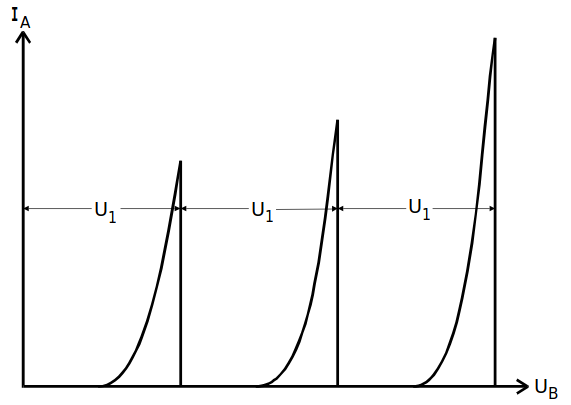
\includegraphics[width=12.0cm]{bild2.png}
    \caption{Absorptionskoeffzienten in Abhängigkeit von der Energie für die jeweilligen Wechselwirkungsprozesse. \cite{quelle01}}
    \label{fig:tfig2}
\end{figure}
\FloatBarrier
\noindent

\subsection{\texorpdfstring{$\beta$}{}-Strahlung}
$\beta$-Strahlung besteht aus Elektronen und ensteht bei dem Zerfall eines Atomkerns. Bei diesem zerfällt ein Neutron $n$ in ein
Proton $p$, ein Elektron $\beta^{-}$ und ein Antineutrino $\bar{\nu}_{\symup{e}}$, nach der Gleichung
\begin{equation}
n \rightarrow p+\beta^{-}+\bar{\nu}_{\symup{e}} \quad .
\end{equation}
Die freigesetzte Energie verteilt sich statistisch auf das Elektron und das Neutrino. Somit kann die Energie des $\beta$-Teilchen
beliebige Werte annehmen, die kleiner oder gleich der bei dem Pozess freiwerdenen Energie sind. Daher ist das Spektrum des $\beta$-Strahlers
kontinuierlich.

Trifft ein $\beta$-Teilchen auf Materie kommt es aufgrund ihrer Ladung zu Wechselwirkungen. Eines dieser Wechselwirkungsprozesse ist die
\textit{Rutherford-Streuung}, bei welcher die $\beta$-Teilchen durch das Elektrische Feld der Kerne eine Richtungsänderung erfahren und somit die Intensität abnimmt.
Außerdem wird durch die Richtungsänderung die Bahn der Teilchen in der Materie verlängert, sodass die tatsächliche Reichweite nicht der Eindringtiefe in das Medium entspricht.
Zwar ist die Energieabnahme durch die Rutherford-Streuung relativ gering, jedoch kann eine Auffächerung des Strahls durch die Richtungsänderung der $\beta$-Teilchen beobachtet werden.

Ein weiterer Prozess, wecher die $\beta$-Teilchen beeinflusst, ist die \textit{inelastische Streuung} am Atomkern. Bei diesem werden die geladenen $\beta$-Teilchen
durch das elektrische Feld der Atomkerne beschleunigt und geben durch diese Beschleunigung elektromagnetische Strahlung ab, was für die Teilchen wiederum einen Energieverlust bedeutet.
Da das Elektron durch die Strahlung abgebremst wird, wird diese Strahlung auch Bremsstrahlung genannt.
Der Wirkungsquerschnitt dieses Prozesses ist durch
\begin{equation}
\sigma_{\text{Br}}=\alpha r_{\text{e}}^2Z^2
\end{equation}
gegeben, wobei $\alpha$ die Sommerfeldsche Feinstrukturkonstante ist.

Inelastische Streuung der $\beta$-Teilchen findet auch an den Elektronen des Absorbermaterials statt, was zu Ionisation und Anregung der Absorberatome führt.
Da bei einem dieser Prozesse nicht die gesamte Energie des $\beta$-Teilchens verbraucht wird, kann es mehrere Wechselwirkungen dieser Art vollziehen bis es vollständig abgebremst ist.
Der Energieverlust pro Absorberschichtdicke ist durch
\begin{equation}
\frac{\symup{d}E}{\symup{d}x}\approx \frac{2\pi r_{\text{e}}^2}{E_{\beta}}\frac{N_{\text{A}}\rho}{M}Z\ln{\frac{E_{\beta}}{I}}
\end{equation}
gegeben.
Auch die Absorptionskurve des $\beta$-Strahlers zeigt, so wie die des $\gamma$-Strahlers, einen exponentiellen Abfall. Allerdings gilt das exponentielle Absorptionsgesetz für
Schichtdicken, die etwa der maximalen Reichweite entsprechen, nicht mehr, da im Bereich hinter der maximalen Reichweite die gemessene Strahlung nicht der $\beta$-Strahlung sondern
der Bremstrahlung oder der kosmischen Hintergrundstrahlung entspricht. 

\FloatBarrier
\begin{figure}[h]
    \centering
    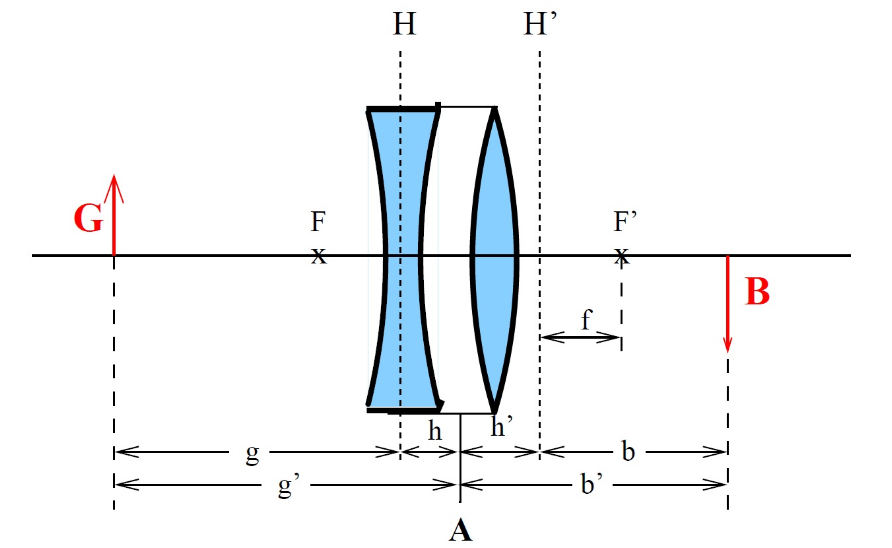
\includegraphics[width=12.0cm]{bild4.png}
    \caption{Absortionskurve eines $\beta$-Strahlers. \cite{quelle01}}
    \label{fig:tfig3}
\end{figure}
\FloatBarrier
\noindent
In Abbildung \ref{fig:tfig3} ist die Absorptionskurve eines $\beta$-Strahlers zu sehen. Aufgetragen ist die logarithmierte Strahlungsintensität in Abhängigkeit von der Massebelegung
\begin{equation}
R=\rho D
\end{equation}
des Absorbers. Aus der maximalen Massebelegung 
$R_{\text{max}}$ kann die gesamte bei dem Zerfall freiwerdende Energie $E_{\text{max}}$ durch
\begin{equation}
    \label{eq:emax}
E_{\text{max}}=1,92\sqrt{R_{\text{max}}^2+0,22R_{\text{max}}} [\symup{MeV}]
\end{equation}
berechnet werden.


\section{Durchführung}
Der Aufbau des Versuches zur Untersuchung der $\gamma$-Strahlung ist schematisch in Abbildung \ref{fig:tfig4} dargestellt.
Aus Sicherheitsgründen und um den Nullfluss zu minimieren ist die Apperatur, die zur Messung der $\gamma$-Strahlung dient, 
von Bleiblöcken umgeben. Die Apperatur zur Untersuchung der $\beta$-Strahlung ist durch Aluminium abgeschirmt. 
Durch ein Geiger-Müller-Zählrohr wird die Strahlungsintensität
registriert. Die Messdauer kann mittels eines Zählwerks variiert werden.
Als $\gamma$-Strahlungsquelle wurde $^{137}$Cs und als $\beta$-Strahlungsquelle $^{99}$Tc verwendet.

\FloatBarrier
\begin{figure}[h]
    \centering
    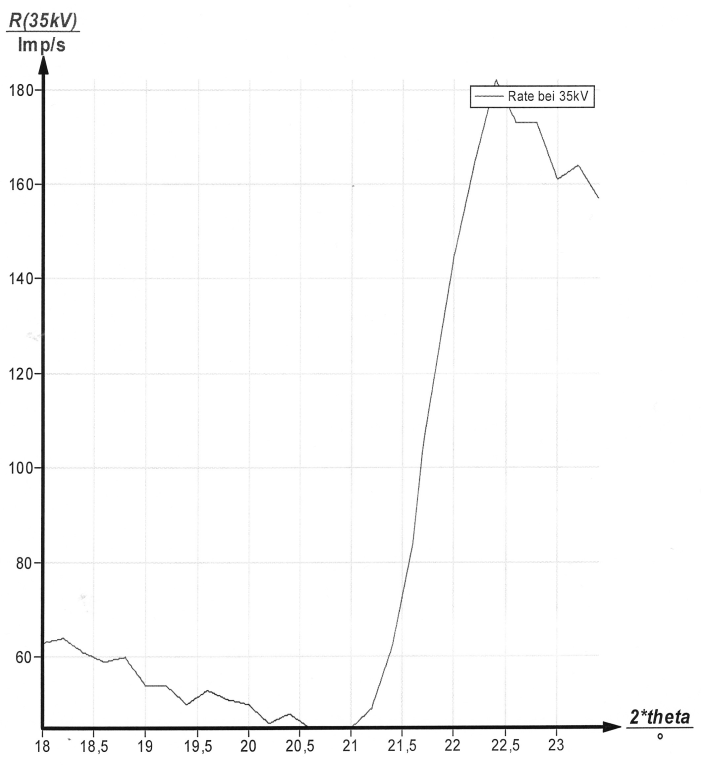
\includegraphics[width=12.0cm]{bild5.png}
    \caption{Versuchsaufbau zur Untersuchung der $\gamma$-Strahlung. \cite{quelle01}}
    \label{fig:tfig4}
\end{figure}
\FloatBarrier

Zu Beginn wird $\SI{900}{\s}$ lang eine Nullmessung, also eine Messung ohne Strahlungsquelle, durchgeführt.
Für die Untersuchung der Absorption von $\gamma$-Strahlung wird ein Absorber mit einer Dicke von $\SI {0,5}{\cm}$ zwischen
Strahlungquelle und Zählrohr platziert und eine $\SI{60}{\s}$-Messung durchgeführt. Die Dicke des Absorbers wird in $\SI{0,5}{\cm}$ Schritten
erhöht, bis sie $\SI{5}{\cm}$ beträgt. Die Messdauer wird für dickere Absorber ebenfalls erhöht. Dieses Verfahren wird für Blei und Eisen durchgeführt, wobei
die Zähldauer bei Blei bis auf $\SI{600}{\s}$ und bei Eisen bis auf $\SI{300}{\s}$ erhöht wird.

Für die Messung der $\beta$-Strahlung werden elf Aluminium Platten mit einer Dicke zwischen $\SI{}{\cm}$ und $\SI{}{\cm}$ untersucht. Die Messdauer
variiert hierbei zwischen $\SI{}{\s}$ und $\SI{}{\s}$ je nach Dicke der Platte.

\section{Auswertung}
\subsection{Messung des Nulleffekts}
Die Ergebnisse der Messung des Nulleffekts sind in Tabelle \ref{tab:atab1} aufgeführt. 
\FloatBarrier
\begin{table}[h]
    \centering
    \caption{Messwerte des Nulleffekts zur Korrektur der Messung zu $\gamma$- und $\beta$-Strahlung.}
    \label{tab:atab1}
    \begin{tabular}{l S[table-format=3.0] S[table-format=3.0] @{${}\pm{}$} S[table-format=2.2] S[table-format=1.3] @{${}\pm{}$} S[table-format=1.3]}
        \toprule
        {} & {$t / \, \si{\second}$} & \multicolumn{2}{c}{$N$} & \multicolumn{2}{c}{$\frac{N}{t} \, / \, \frac{1}{\si{\second}}$} \\
        \midrule
        {$\gamma$-Strahlung} & 900 & 973 & 31,19 & 1,081 & 0,035 \\
        {$\beta$-Strahlung}  & 900 & 551 & 23    & 0,61  & 0,03  \\
        \bottomrule
    \end{tabular}
\end{table}
\FloatBarrier
\noindent
Da die Messung der Zählrate $N$ der Poisson-Verteilung unterliegt, ergibt sich ein Fehler $\sqrt{N}$. Dieser Fehler wirkt sich auch
auf die Ergebnisse der Zählrate pro Zeiteinheit $\frac{N}{t}$ aus und errechnet sich über die Gauß'sche Fehlerfortpflanzung, 
die mit \texttt{Python 3.6.5} \cite{quelle02} und \texttt{uncertainties} \cite{quelle03} durchgeführt wird.

\subsection{\texorpdfstring{$\gamma$}{}-Strahlung}
Die Messwerte zur Messung des Absorptionskoeffizienten von Blei sind in Tabelle \ref{tab:atab2} aufgeführt. 
\FloatBarrier
\begin{table}[h]
    \centering
    \caption{Messwerte zur Bestimmung des Absorptionskoeffizienten $\mu_\text{Pb}$ und der Größe $N\left(0\right)$ von Blei.}
    \label{tab:atab2}
    \begin{tabular}{S[table-format=1.3] S[table-format=3.0] S[table-format=4.0] @{${}\pm{}$} S[table-format=2.2] S[table-format=2.2] @{${}\pm{}$} S[table-format=1.2]}
        \toprule
        {$d / \, \si{\meter}$} & {$t / \, \si{\second}$} & \multicolumn{2}{c}{$N$} & \multicolumn{2}{c}{$\; \; \frac{N}{t} \, / \, \frac{1}{\si{\second}}$} \\
        \midrule
        0,005 & 60  & 5016 & 70,82 & 82,52 & 1,18 \\
        0,010 & 120 & 5760 & 75,90 & 46,92 & 0,63 \\
        0,015 & 180 & 4680 & 68,41 & 24,92 & 0,38 \\
        0,020 & 240 & 3907 & 62,51 & 15,20 & 0,26 \\
        0,025 & 300 & 3121 & 55,87 & 9,32  & 0,19 \\
        0,030 & 360 & 2415 & 49,14 & 5,63  & 0,14 \\
        0,035 & 420 & 1730 & 41,59 & 3,04  & 0,10 \\
        0,040 & 480 & 1428 & 37,79 & 1,89  & 0,09 \\
        0,045 & 540 & 1270 & 35,64 & 1,27  & 0,07 \\
        0,050 & 600 & 971  & 31,16 & 0,54  & 0,06 \\
        \bottomrule
    \end{tabular}
\end{table}
\FloatBarrier
\noindent
Diese Messwerte der Zählrate pro Zeiteinheit $\frac{N}{t}$ sind in Abbildung \ref{fig:afig1} halblogarithmisch gegen 
die Dicke $d$ des Absorbermaterials ausgetragen. Die Korrektur die sich aus der Nullmessung ergibt, ist als Fehlerbalken
an den einzelnen Messwerten dargestellt. Mit einer linearen Ausgleichsrechnung ergeben sich die Parameter
\begin{align*}
    a &= \num{-107,635(2317)} \, \frac{1}{\si{\meter}} \\
    b &= \num{4,912(72)}      \, \frac{1}{\si{\second}} \,
\end{align*}
wobei $a$ den Absorptionskoeffizienten von Blei $\mu_\text{Pb}$ und $b$ die Größe $N\left(0\right)$ als Anzahl der eintreffenden
Teilchen pro Zeiteinheit ohne Absorber darstellt. 
\FloatBarrier
\begin{figure}[h]
    \centering
    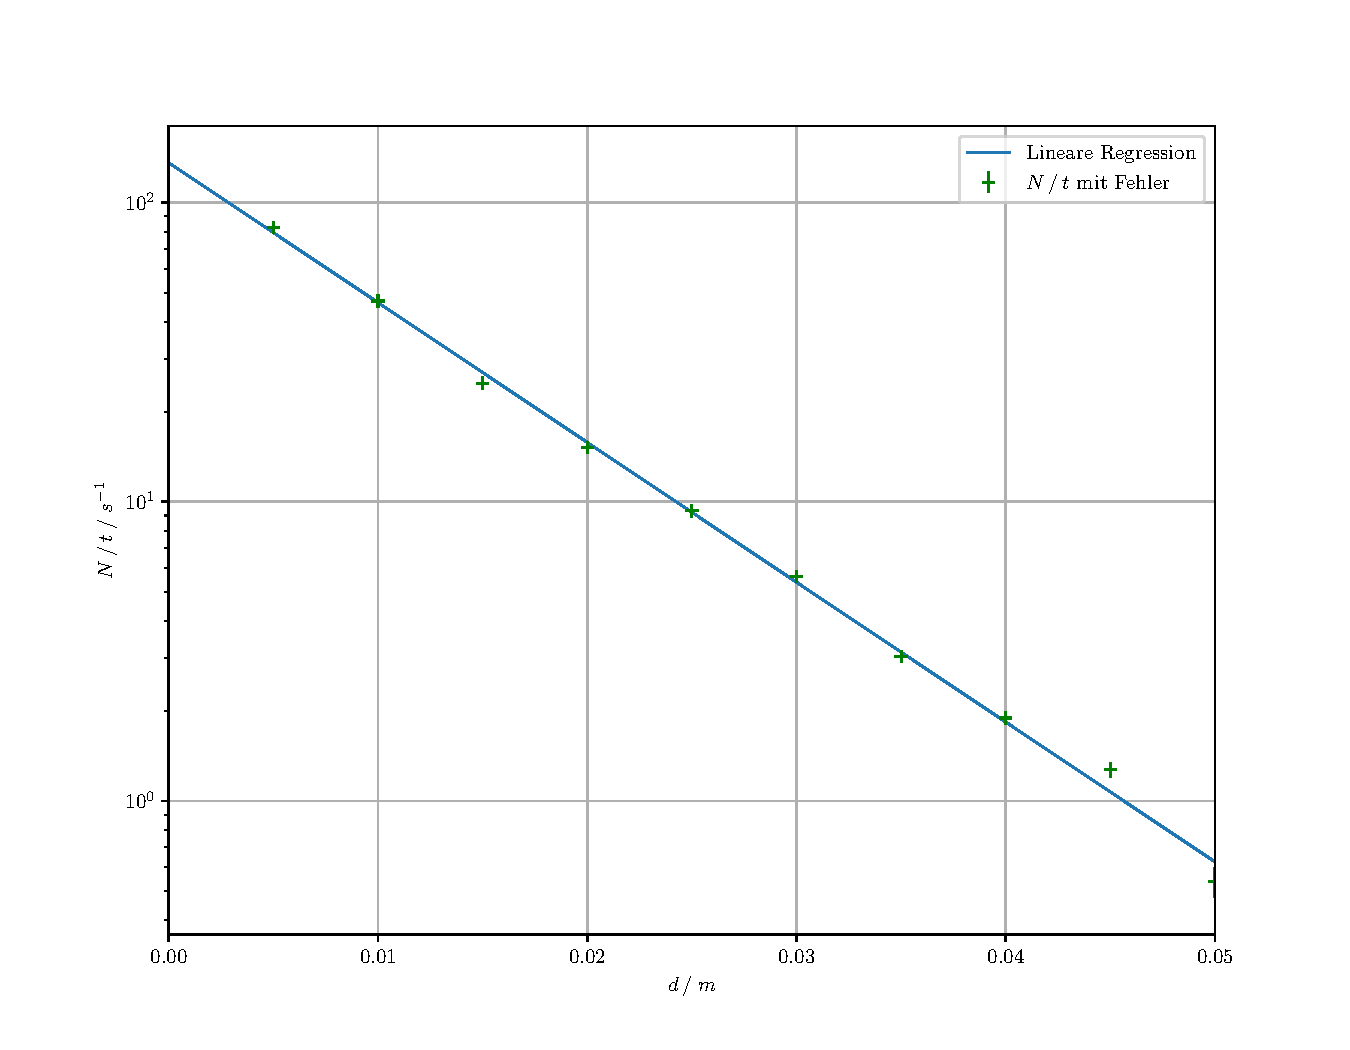
\includegraphics[width=13.5cm]{blei.pdf}
    \caption{Lineare Ausgleichsrechung zur Bestimmung des Absorptionskoeffizienten $\mu_\text{Pb}$ und der Größe $N\left(0\right)$ von Blei. 
    Dargestellt ist die Zählrate $N$ pro Zeiteinheit $t$ in Abhängigkeit von der Dicke $d$.}
    \label{fig:afig1}
\end{figure}
\FloatBarrier
\noindent
Die Bestimmung des Absorptionskoeffizienten von Eisen $\mu_\text{Fe}$ erfolgt analog. Die Messwerte dieser Messung sind
in Tabelle \ref{tab:atab3} dargestellt.
\FloatBarrier
\begin{table}[h]
    \centering
    \caption{Messwerte zur Bestimmung des Absorptionskoeffizienten $\mu_\text{Fe}$ und der Größe $N\left(0\right)$ von Eisen.}
    \label{tab:atab3}
    \begin{tabular}{S[table-format=1.3] S[table-format=3.0] S[table-format=4.0] @{${}\pm{}$} S[table-format=2.2] S[table-format=3.2] @{${}\pm{}$} S[table-format=1.2]}
        \toprule
        {$d / \, \si{\meter}$} & {$t / \, \si{\second}$} & \multicolumn{2}{c}{$N$} & \multicolumn{2}{c}{$\; \; \frac{N}{t} \, / \, \frac{1}{\si{\second}}$} \\
        \midrule
        0,005 & 60  & 6853 & 82,78 & 113,14 & 1,38 \\
        0,010 & 90  & 8167 & 90,37 & 89,66  & 1,00 \\
        0,015 & 120 & 8208 & 90,60 & 67,32  & 0,76 \\
        0,020 & 150 & 8078 & 89,88 & 52,77  & 0,60 \\
        0,025 & 170 & 8142 & 90,23 & 46,81  & 0,53 \\
        0,030 & 190 & 6997 & 83,65 & 35,75  & 0,44 \\
        0,035 & 210 & 6030 & 77,65 & 27,63  & 0,37 \\
        0,040 & 240 & 5674 & 75,33 & 22,56  & 0,32 \\
        0,045 & 270 & 5028 & 70,91 & 17,54  & 0,26 \\
        0,050 & 300 & 4661 & 68,27 & 14,46  & 0,23 \\
        \bottomrule
    \end{tabular}
\end{table}
\FloatBarrier
\noindent
Aus der linearen Ausgleichsrechnung in Abbildung \ref{fig:afig2} ergeben sich so die Parameter 
\begin{align*}
    a &= \num{-45,594(873)} \, \frac{1}{\si{\meter}}\\
    b &= \num{4,933(27)} \, \frac{1}{\si{\second}} \quad .
\end{align*}
\FloatBarrier
\begin{figure}[h]
    \centering
    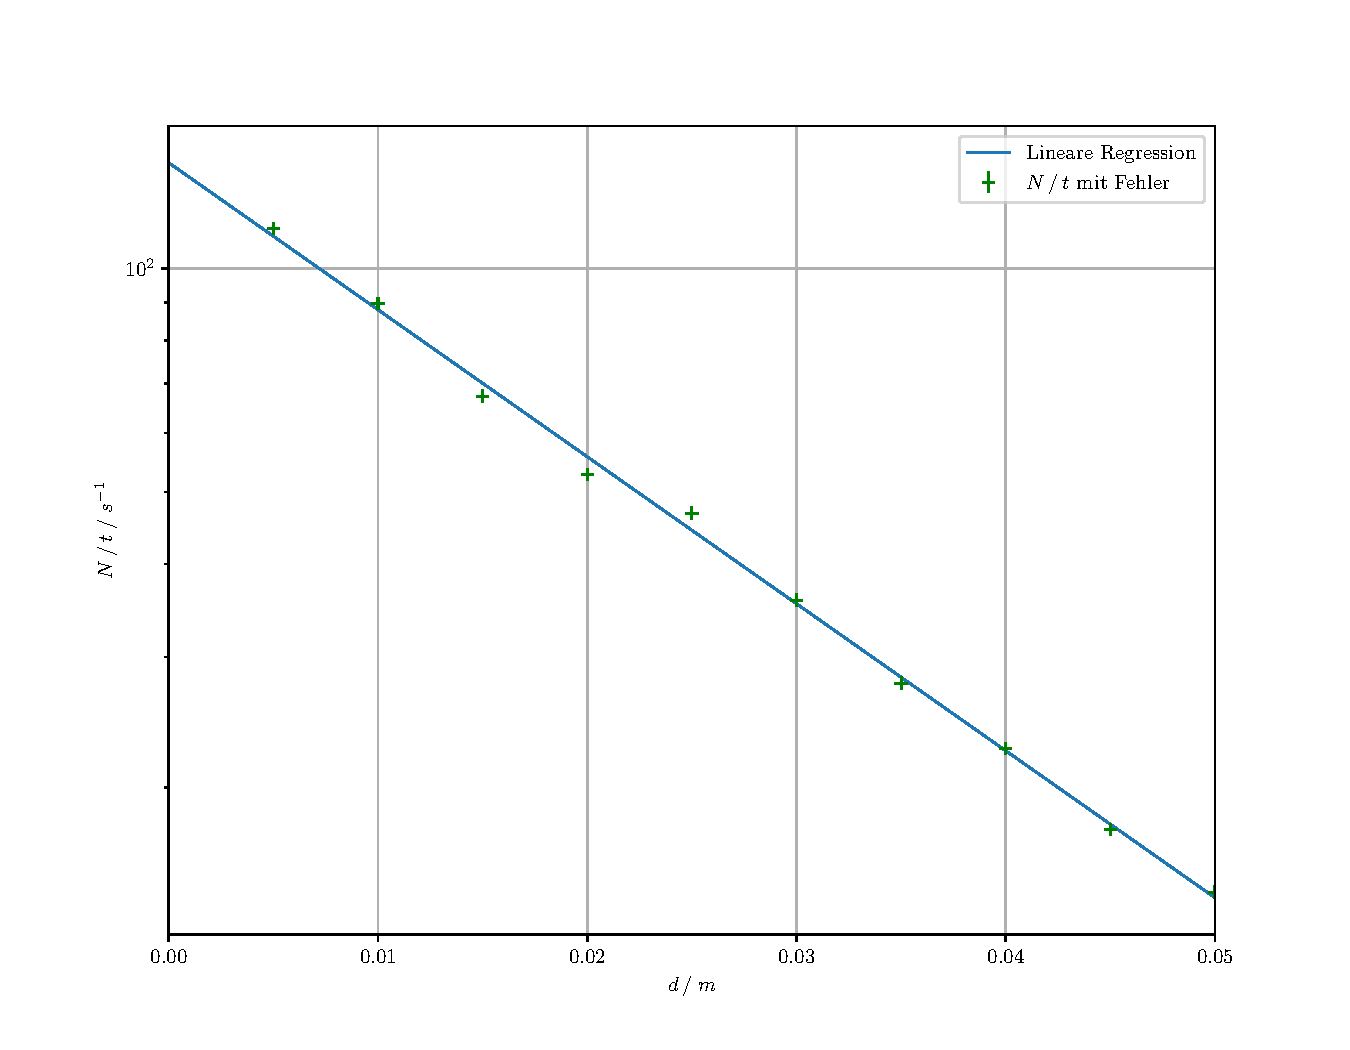
\includegraphics[width=13.5cm]{eisen.pdf}
    \caption{Lineare Ausgleichsrechung zur Bestimmung des Absorptionskoeffizienten $\mu_\text{Fe}$ und der Größe $N\left(0\right)$ von Eisen. 
    Dargestellt ist die Zählrate $N$ pro Zeiteinheit $t$ in Abhängigkeit von der Dicke $d$.}
    \label{fig:afig2}
\end{figure}
\FloatBarrier

\subsubsection{Berechnung des Absorptionskoeffizienten \texorpdfstring{$\mu_\text{Compton}$}{}}
Als Vergleichswert für die experimentell ermittelten Werte der Absorptionskoeffizienten von Blei und Eisen wird aus
Formel \eqref{eq:mucompton} der Compton-Absorptionskoeffizient $\mu_\text{Compton}$ bestimmt. Dazu muss der Wirkungsquerschnitt
der Compton-Streuung $\sigma_\text{Compton}$ für $\ce{^{137}Cs}$ bekannt sein, der sich aus Formel \eqref{eq:sigmacompton} und dem 
Energieverhältnis $\varepsilon = 1.295$ berechnet, sodass folgt
\begin{equation*}
    \sigma_\text{Compton} = \SI{2,566e-29}{\meter\squared} \quad .
\end{equation*}
Mit den stoffspezifischen Werten in Tabelle \ref{tab:atab4} ergibt sich so für den Absorptionskoeffizienten $\mu_\text{Compton}$
\begin{align*}
    \mu_\text{Compton, Pb} &= 69,351 \, \frac{1}{\si{\meter}} \\
    \mu_\text{Compton, Fe} &= 56,640 \, \frac{1}{\si{\meter}} \quad .
\end{align*}
\FloatBarrier
\begin{table}[h]
    \centering
    \caption{Stoffspezifische Werte zur Berechnung des Absorptionskoeffizienten $\mu_\text{Compton}$ \cite{quelle04}.}
    \label{tab:atab4}
    \begin{tabular}{l c c  S[table-format=1.4]}
        \toprule
        {} & {$Z$} & {$\rho / \, \si[per-mode=reciprocal]{\kilo\gram\per\cubic\meter}$} & {$M / \, \si[per-mode=reciprocal]{\kilo\gram\per\mol}$} \\
        \midrule
        {Blei}  & 82 & 11342 & 0,2072 \\
        {Eisen} & 26 & 7874  & 0,0558 \\
        \bottomrule
    \end{tabular}
\end{table}
\FloatBarrier


\subsection{\texorpdfstring{$\beta$}{}-Strahlung}
Die Messwerte zur Bestimmung der Maximalenergie $E_\text{max}$ der $\beta$-Strahlungsquelle $\ce{^{99}Te}$ sind in 
Tabelle \ref{tab:atab5} dargestellt.
\FloatBarrier
\begin{table}[h]
    \centering
    \caption{Messwerte zur Bestimmung der Maximalenergie $E_\text{max}$ der $\beta$-Strahlungsquelle $\ce{^{99}Te}$.}
    \label{tab:atab5}
    \begin{tabular}{S[table-format=3.0] S[table-format=4.0] S[table-format=5.0] @{${}\pm{}$} l S[table-format=3.4] @{${}\pm{}$} S[table-format=1.4]}
        \toprule
        {$d / \, \SI{e-6}{\meter}$} & {$t / \, \si{\second}$} & \multicolumn{2}{c}{$N$} & \multicolumn{2}{c}{$\; \; \frac{N}{t} \, / \, \frac{1}{\si{\second}}$} \\
        \midrule
        482 & 1100 & 774   & 27,82 & 0,0914   & 0,0360 \\
        444 & 1000 & 683   & 26,13 & 0,0708   & 0,0366 \\
        400 & 900  & 642   & 25,34 & 0,1011   & 0,0380 \\
        338 & 800  & 494   & 22,23 & 0,0053   & 0,0377 \\
        302 & 700  & 505   & 22,47 & 0,1092   & 0,0410 \\
        253 & 600  & 501   & 22,38 & 0,2228   & 0,0452 \\
        200 & 500  & 794   & 28,18 & 0,9758   & 0,0619 \\
        160 & 400  & 1704  & 41,28 & 3,6478   & 0,1063 \\
        153 & 300  & 2037  & 45,13 & 6,1778   & 0,1526 \\
        125 & 200  & 1439  & 37,93 & 6,5828   & 0,1914 \\
        100 & 100  & 2747  & 52,41 & 26,8578  & 0,5247 \\
        0   & 50   & 22220 & 149,0 & 443,7878 & 2,9814 \\
        \bottomrule
    \end{tabular}
\end{table}
\FloatBarrier
\noindent
Die Fehlerrechnung erfolgt hierbei analog zum ersten Auswertungsteil zu $\gamma$-Strahlung. In Abbildung \ref{fig:afig3}
sind die Messwerte der Zählrate pro Zeiteinheit $\frac{N}{t}$ mit ihrem Fehler gegen die Dicke $d$ aufgetragen. 
\FloatBarrier
\begin{figure}[h]
    \centering
    \includegraphics[width=13.5cm]{betastrahlung.pdf}
    \caption{Lineare Ausgleichsrechung zur Bestimmung der Maximalenergie $E_\text{max}$ der $\beta$-Strahlungsquelle $\ce{^{99}Tc}$. 
    Dargestellt ist die Zählrate $N$ pro Zeiteinheit $t$ in Abhängigkeit von der Dicke $d$.}
    \label{fig:afig3}
\end{figure}
\FloatBarrier
\noindent
Mit zwei linearen Ausgleichsrechnungen für die Werte oberhalb und unterhalb des Schnittpunkts $R_\text{max}$ ergeben
sich die Parameter
\begin{align*}
    a_1 &= \num{-29715,658(4560767)} \, \frac{1}{\si{\meter}} & a_2 &= \num{-1079,148(10454891)} \, \frac{1}{\si{\meter}} \\
    b_1 &= \num{6,074(557)} \, \frac{1}{\si{\second}}         & b_2 &= \num{2,316(3956)} \, \frac{1}{\si{\second}} \; .
\end{align*}
Aus diesen Parametern kann mit der Beziehung
\begin{equation*}
    R_{\text{max}} = \frac{b_2 - b_1}{a_1 - a_2} \cdot \rho_\text{Al}
\end{equation*}
die maximale Massenbelegung berechnet werden, die der $x$-Koordinate des Schnittpunkts der beiden Ausgleichsgeraden entspricht.
Es ergibt sich 
\begin{equation*}
    R_{\text{max}} = \num{0.794(493)} \, \si{\kilo\gram\per\meter} \; ,
\end{equation*}
sodass aus Formel \eqref{eq:emax} die Maximalenergie des $\ce{^{99}Tc}$ 
\begin{equation*}
    E_\text{max}  = \num{0.296(116)} \, \si{\mega\electronvolt}
\end{equation*}
folgt.

\section{Diskussion}
Zur besseren Übersicht der Ergebnisse sind die experimentell und theoretisch bestimmten Werte der Absorptionskoeffizienten
mit der jeweiligen Abweichung in Tabelle \ref{tab:dtab1} dargestellt.
\FloatBarrier
\begin{table}[h]
    \centering
    \caption{Experimentell und theoretisch bestimmte Werte der Absorptionskoeffizienten von Blei und Eisen.}
    \label{tab:atab2}
    \begin{tabular}{l S[table-format=3.3] @{${}\pm{}$} S[table-format=1.4] S[table-format=2.3] S[table-format=2.2]}
        \toprule
        {} & \multicolumn{2}{c}{$\mu_\text{Experiment} / \, \si[per-mode=reciprocal]{\per\meter}$} & {$\mu_\text{Compton} / \, \si[per-mode=reciprocal]{\per\meter}$} & {Abweichung / \%} \\
        \midrule
        {Blei}  &  -107,635 & 2,317 & 69,351 & 55,20 \\
        {Eisen} &  -45,594  & 0,873 & 56,640 & 21,27 \\
        \bottomrule
    \end{tabular}
\end{table}
\FloatBarrier
\noindent
Die Werte des experimentell bestimmten Absorptionskoeffizienten von Blei und Eisen weichen deutlich von den berechneten
Werten der Absorptionskoeffizienten $\mu_\text{Compton}$ ab. Die dieser in beiden Fällen unterhalb des experimentell 
bestimmten Wertes liegt, ist zu schlussfolgern, dass bei dieser Messung der Photoeffekt der dominierende Absorptionsmechanismus ist. 
Die Werte von $N(0) = \num{4,912(72)} \, \si[per-mode=reciprocal]{\per\second}$ für Blei und $N(0) = \num{4,933(27)} \, \si[per-mode=reciprocal]{\per\second}$
für Eisen unterscheiden sich mit einer Abweichung von 0,43\% nur geringfügig, was auf eine hohe Genauigkeit der Messung schließen lässt.
Messfehler können jedoch durch das verwendete Absorbermaterial entstanden sein, welches möglicherweise nicht überall
die gleiche Dicke aufweist. 

Da keine Vergleichswerte für die Ergebnisse der Messung zur $\beta$-Strahlung vorliegen, ist eine qualitative Diskussion
der Ergebnisse an dieser Stelle nicht möglich. Mögliche Messfehler können jedoch bei beiden Messungen durch längere
Messzeiten verringert werden.

\nocite{wingate}   
\nocite{*}      
\printbibliography

\end{document}